
\section{The Room Without a Name}

\subsection{The Architecture of Deniability}

A few days later, David caught a text message from Hart.

\begin{quote}
  Dinner next week at the Observatory. Paolo from the regulator’s office will be there. You remember him from the club 
  last month? He’s already excited about the model. Want me to give him a heads-up so he’s primed for the conversation?
\end{quote}

There was no explicit ask. There was no leverage spelled out.

The Observatory sounded innocuous enough. On paper, it was an upscale restaurant. It was a place you could legally expense 
dinner, complete with a sommelier, white tablecloths, and a view of the skyline.  

Technically, it wasn’t a gentleman’s club. Technically.

But those who were in the know understood the real layout. The Observatory shared a building --- and an ownership --- with 
``the Velvet'', the adjacent strip club. The parent company quietly operated both, using a labyrinth of shell 
LLCs to keep the relationship opaque.

And tucked between the restaurant’s wine cellar and the Velvet’s private booths was a “large private room” — soundproofed, 
dimly lit, and sunken just enough to feel separate from the world above. On the restaurant side, it was accessible through 
a discreet door past the cellar. On the club side, it connected to a mirrored lounge behind the Velvet’s VIP booths — a 
room with a semicircular sofa that opened in the middle to reveal a hidden door.

That door was the point. It allowed the girls from the club to join guests from the restaurant without ever passing through 
the main floor. They entered quietly, unannounced, as if part of the ambiance. 

\medskip

\begin{figure}[H]
  \centering
  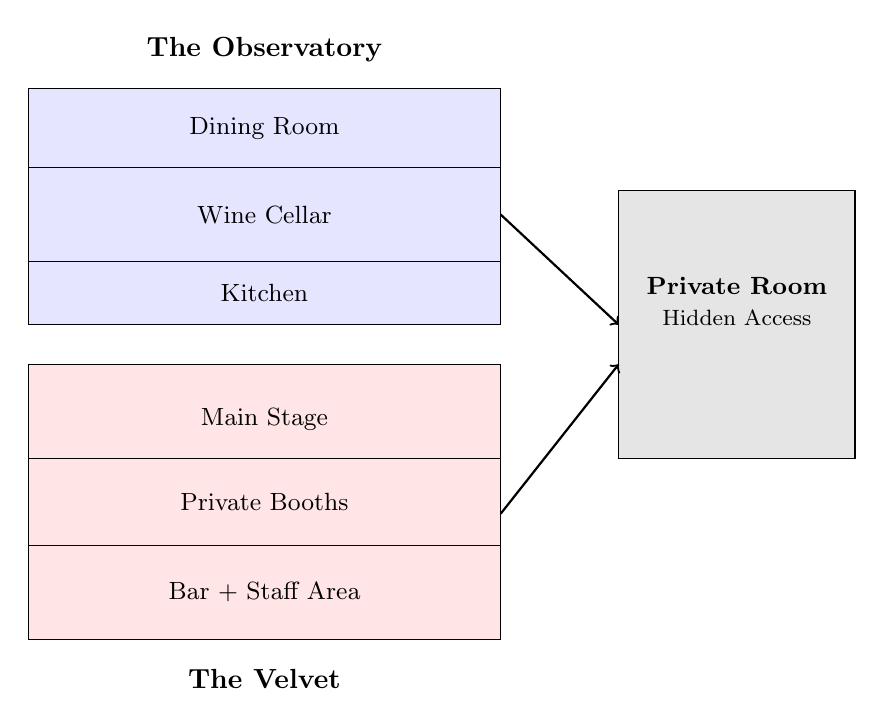
\begin{tikzpicture}[scale=1, font=\small]
  
    % === FLOOR PLAN ===
  
    % The Observatory — 1st Floor Layout
    \draw[fill=blue!10] (0,4) rectangle (6,7); % Restaurant
    \node[font=\bfseries] at (3.0, 7.5) {The Observatory};
    \draw (0,6) -- (6,6); % Divider line
    \node at (3,6.5) {Dining Room};
    \draw (0,4.8) -- (6,4.8);
    \node at (3,5.4) {Wine Cellar};
    \node at (3,4.4) {Kitchen};
  
    % The Velvet — Basement Layout
    \draw[fill=red!10] (0,0) rectangle (6,3.5); % Club
    \node[font=\bfseries] at (3,-0.5) {The Velvet};
    \draw (0,2.3) -- (6,2.3);
    \node at (3,2.8) {Main Stage};
    \draw (0,1.2) -- (6,1.2);
    \node at (3,1.75) {Private Booths};
    \node at (3,0.6) {Bar + Staff Area};
  
    % Shared Private Room
    \draw[fill=gray!20] (7.5,2.3) rectangle (10.5,5.7); 
    \node[align=center] at (9,4.3) {\textbf{Private Room}\\\footnotesize Hidden Access};
  
    % Entry arrows to Private Room
    \draw[->, thick] (6,5.4) -- (7.5,4.0); % From wine cellar
    \draw[->, thick] (6,1.6) -- (7.5,3.5); % From booths
  
    % === CORPORATE STRUCTURE ===
    %\node[font=\bfseries] at (15,8.5) {Corporate Ownership Structure};
  
    % Parent company
    %\draw[fill=black!5] (13,7.8) rectangle (17,8.3);
    %\node at (15,8.05) {\textbf{Orion Hospitality Group, LLC}};
  
    % Shells
    %\draw[fill=black!10] (13,6.8) rectangle (17,7.3);
    %\node at (15,7.05) {Shell LLC A — The Velvet};
  
    %\draw[fill=black!10] (13,5.6) rectangle (17,6.1);
    %\node at (15,5.85) {Shell LLC B — The Observatory};
  
    %\draw[fill=black!10] (13,4.4) rectangle (17,4.9);
    %\node at (15,4.65) {Shell LLC C — Private Room};
  
  \end{tikzpicture}
  \caption{
    Architectural floor plan of The Observatory (restaurant), The Velvet (club), and a hidden shared private 
    room — all legally separated by distinct shell LLCs but operated under a single parent entity.
  }
\end{figure}
  
\medskip 

The girls were not staff. But they were not exactly guests, either. The girls were just close 
enough to blur the line, and just far enough to keep anything that happened off the books.

The room itself was equal parts seduction and strategy. On the far side, a 
large circular bed 
slowly revolved under soft amber lights, not fast enough to draw attention, but just enough to suggest movement even when no 
one was on it. Opposite that, a narrow staircase led up to a small balcony lounge with low armchairs and a view that looked 
down over everything: the bed, the tables, and the guests. From up there, the whole scene played like theater.

Beneath the balcony sat a tastefully integrated dancer’s pole that was polished to a mirror finish.
Between the pole and the bed, a row of dark walnut tables offered just enough space for a whiskey flight.
Leather-backed chairs, matte black sugar trays, flickering votives completed the setup, and evoked a high-end coffee shop 
more than a club. It gave cover to whatever the guests chose to call the evening.


After dessert, it wasn’t uncommon for the night to 
migrate there.  Sometimes the wives joined. Sometimes they didn’t.  Sometimes 
they brought their own guests.  On the expense report, it was just a dinner.  It was just a networking event.  
It was just a hospitality line item.  But everyone understood. What happened in the private room wasn’t on the receipt.  
But it was part of the bargain.

If anything compromising happened in that room — a lapse in judgment, a moment of indulgence, a scene that didn’t belong 
in a compliance report — it wouldn’t trace back to the restaurant or the club. Not directly.

The layout made that possible. And so did the paperwork.

The private room acted like a firewall. It was where someone could have a ``business dinner'', and no one would ask questions. 
The circular bed wasn’t just for show, and the mirrored ceiling above it wasn’t an accident. 
Security staff knew where to turn the cameras, and the exit to the Velvet was marked only from the inside. 

\medskip

\begin{TechnicalSidebar}{Significance of a Shell LLC Leasing the Private Room}

  The decision to lease the private room under a shell company wasn’t just legal 
  hygiene. It was structural intent.

  \medskip
  
  First, it created containment. If anything controversial or reputationally toxic happened behind those doors — 
  a lapse in decorum, a breach of ethics, even a crime — liability wouldn’t touch the restaurant or the club. Not 
  directly. On paper, the room belonged to a “private event services firm,” a neutral tenant with no obvious 
  connection to adult entertainment or fine dining. To regulators, auditors, or journalists, the room became a 
  dead end in the org chart.

  \medskip
  
  That insulation granted flexibility. The space could serve multiple roles depending on who was asking. From the 
  restaurant’s side, it might be described as a wine cellar annex or executive dining suite. From the club’s side, 
  it could be pitched as VIP overflow, though never formally listed as part of the venue. And if the conversation 
  was too delicate for either brand to claim, the room could simply be leased out to “external partners” — a 
  euphemism everyone understood.

  \medskip
  
  Then came the deniability. If subpoenas arrived or FOIA requests were filed, staff could answer with complete 
  honesty: that room wasn’t under their control. Access logs, contracts, and invitations all pointed elsewhere. 
  The ambiguity wasn’t a flaw in the structure. It was the feature.

  \medskip
  
  But the real power came in access management. Because the room sat in the jurisdiction of a separate LLC, so 
  did its entry permissions. Key cards, security footage, guest lists were all handled through a different custodial 
  layer. It became a liminal space: technically private, legally detached, and socially malleable. Only insiders 
  understood how fluid the boundary really was.

  \medskip
  
  And finally, there was the financial dimension. A standalone LLC could receive funding through hospitality budgets, 
  bill clients under consulting fees, or depreciate the cost of “client engagement.” Revenues could be rerouted. 
  Expenses could be categorized to fit the desired story. And most importantly, any paper trail would read like a 
  footnote in someone else’s ledger.

  \medskip
  
  This wasn’t just about hiding things. It was about structuring optionality. It was not secrecy for its own sake, 
  but mobility. The kind of mobility that made denial credible, audit trails blurry, and influence hard to trace.
  
\end{TechnicalSidebar}

\medskip

\subsection{The Architecture of Mutual Compromise}


But sex wasn’t the only reason the room existed. That was just the cover.

Its real value came when that same room became the setting for off-calendar meetings. Regulators took calls on encrypted 
phones while pretty girls sat on their laps. Vendors pitched exclusivity clauses without lawyers present. A government 
liaison once reviewed a demo on a tablet between dances.

By law, to avoid conflicts of interest, to preserve impartiality, and to maintain the appearance of independence,
there are situations where \textbf{regulators, auditors, and clients aren’t allowed to share the same room outside
official business}.

But no statute prohibits a regulator from dining at the Observatory, or a client from entering the Velvet. And if they 
happened to meet in the private room? Well, that was just coincidence.

And everyone who entered the room had skin in the game. The cameras weren’t official, but the girls had seen your face. No 
one said it aloud, but the room made sure that what happened there stayed off the record. It made people speak differently. 
It made them speak more candidly. And it made them more open to compromise.


It wasn’t unusual for a portfolio to be rebalanced while someone’s wife “entertained” multiple men on stage as part of 
the deal itself. For those in the know, her ``performance'' 
\footnote{Her performance carried implications far beyond the surface. It wasn’t just erotic; it was managerial.
Iceberg Slim in his autobiography ``PIMP: My Life'' once described how his mentor taught him how to ``keep a bitch under 
control'': beat her, then give her a cold bath. The comfort
that follows pain, he said, rewires the loyalty. ``She'll be so thankful for the comfort that she'll forget that you were 
the one who hurt her'', he said. In BDSM, they call it ``aftercare''.
In elite circles, they call it ``hospitality''. Either way, it’s the same logic: control wrapped in tenderness.
This wasn’t indulgence; it was choreography. A performance staged to remind the room who offered warmth,
and who could take it away. A performance staged to remind the room who could hurt you, and who could help you.
What’s ``abuse'' when you’re poor becomes ``ritual'' when you’re rich.
What’s trashy in public becomes classy behind French doors.}
was a message disguised as a spectacle to prove her husband's loyalty and compliance.

That was the real purpose: deniability and leverage.

Because in rooms like this, the real power wasn’t in what was said.  It was in what no one dared to say aloud.

\medskip

\begin{figure}[H]
  \centering

  % === First row ===
  \begin{subfigure}[t]{0.45\textwidth}
  \centering
  \begin{tikzpicture}
    \comicpanel{0}{0}
      {Old Pimp}
      {Young Pimp}
      {To keep her loyal, hurt her then be the one to comfort her. She'll call it kindness.}
      {(-0.6,-0.6)}
  \end{tikzpicture}
  \caption*{The lesson: control delivered as a kindness.}
  \end{subfigure}
  \hfill
  \begin{subfigure}[t]{0.45\textwidth}
  \centering
  \begin{tikzpicture}
    \comicpanel{0}{0}
      {Old Pimp}
      {Young Pimp}
      {OK. But what will the cops call it?}
      {(0.6,-0.6)}
  \end{tikzpicture}
  \caption*{The suspicion: wondering what name gets printed on the charge sheet.}
  \end{subfigure}

  \vspace{1em}

  % === Second row ===
  \begin{subfigure}[t]{0.45\textwidth}
  \centering
  \begin{tikzpicture}
    \comicpanel{0}{0}
      {Venture Hostess}
      {Private Guest}
      {His wife fucked the whole room. Then they whispered to her, ``You were radiant.''}
      {(-0.6,-0.6)}
  \end{tikzpicture}
  \caption*{The reenactment: how to package power plays as premium hospitality.}
  \end{subfigure}
  \hfill
  \begin{subfigure}[t]{0.45\textwidth}
  \centering
  \begin{tikzpicture}
    \comicpanel{0}{0}
      {Venture Hostess}
      {Private Guest}
      {Is that aftercare... or just classier pimping?}
      {(0.6,-0.6)}
  \end{tikzpicture}
  \caption*{The question: when power hides behind legal definitions.}
  \end{subfigure}

  \caption*{If you file it under ``team development,'' you can make pimping a corporate expense.}
\end{figure}

\medskip

\begin{HistoricalSidebar}{\textbf{Silicon Valley’s Secret Dinners --- The Soft Power Rituals of a Networked Elite}}

    In the social architecture of Silicon Valley, access is everything, but rarely advertised. While venture capital 
    firms publish open calls for innovation, the true currency of power often changes hands in private: over 
    wagyu tartare, low lighting, and non-disclosure agreements.

    \medskip
    
    By the late 2010s, a new pattern had emerged: so-called “secret dinners,” elite invite-only gatherings where 
    founders, investors, and influencersmingled in settings that deliberately blurred the 
    line between business and pleasure. They were not parties in the traditional sense. They were \textbf{filters}.

    \medskip
    
    According to reports in \textit{Brotopia} by Emily Chang and corroborated by investigations in 
    \textit{The New York Times} and \textit{Vanity Fair}, these dinners became informal arenas of 
    vetting: social, sexual, and financial.

    \medskip
    
    Some dinners had clear rules: no phones, no press, and no photos. Others relied on unspoken norms. 
    The architecture of power was dressed in Napa wine and casual hoodies, but the logic was access 
    granted through compliance, charm, or mutual implication.
    
\end{HistoricalSidebar}

    

\medskip


\begin{PhilosophicalSidebar}{The Thumbscrew Principle --- Leveraging Mutual Compromise as Insurance}
In high-stakes consulting, reputational risk isn’t always mitigated through compliance—it’s mitigated through 
\textbf{mutual compromise}.  

\medskip

\textbf{Law 33} from \textit{The 48 Laws of Power} explains the underlying psychology:  

\begin{quote}
Discover each man’s thumbscrew.
\end{quote}

In this context, the thumbscrew isn’t leverage from blackmail—it’s the leverage of \textbf{co-participation}. 
You don’t need to threaten exposure if you’ve already pulled them into the same compromising behaviors. Every 
indulgence, every ethical lapse, and every blurred boundary is an insurance policy.  

\begin{quote}
If everyone’s hands are dirty, no one wants to wash them first.
\end{quote}
\end{PhilosophicalSidebar}

\medskip



  



The brilliance wasn’t coercion.  The brilliance was \textbf{slow entanglement}. 
Entanglement so gradual that no single step felt like a compromise.

The Observatory wasn’t a trap door.  It was a funnel lined in velvet.

\begin{quote}
  The real contract wasn’t signed on paper.  The real contract was the months of rooms you shared.
\end{quote}

Hart’s brilliance wasn’t creating leverage over people. It was creating an ecosystem where 
\textbf{everyone had leverage on everyone else}, and thus, no one dared pull the thread.

\medskip

\begin{HistoricalSidebar}{The Broadcom ``Pond'': Henry Nicholas III and the Velvet Trap}

  In the late 1990s and 2000s, tech billionaire \textbf{Henry Nicholas III}, co-founder of Broadcom, wasn’t just making 
  semiconductor chips—he was making headlines for a hidden world beneath his empire.

  \medskip
  
  According to federal prosecutors and court filings, Nicholas built an underground lair beneath his Laguna Niguel warehouse: 
  a secret cave outfitted with a Jacuzzi for six, an \$18{,}000 handcrafted bar, and an Oriental-themed parlor adorned 
  with rugs, statues, and a four-foot Medusa figure. They called it \textbf{“The Ponderosa”} or \textbf{“The Pond.”} 
  Behind a hidden library wall in his mansion, another secret tunnel led to an underground sports bar and recording 
  studio.

  \medskip
  
  But these weren’t just eccentric architectural choices. These were spaces designed for what court filings described as 
  \textbf{marathon drug-fueled orgies}, mixing cocaine, ecstasy, nitrous oxide, prostitutes, and music from Led Zeppelin 
  and Phil Collins in a surreal, days-long bacchanal.

  \medskip
  
  A former employee described the parties: a black box of cocaine sat atop the bar next to a grinder for crushing rocks 
  into powder. A bartender—whom Nicholas had personally sent to bartending school to perfect his favorite cocktail, the 
  \emph{grasshopper}—served guests as they inhaled “whippets” from metal canisters, later replaced by a full nitrous 
  tank when the guests complained the canisters were too cold.

  \medskip
  
  The parties were exclusive, indulgent, and heavily curated. Clients, employees, regulators, and other VIPs were invited 
  to ``network''. A former assistant alleged he was forced to act as a drug courier and to make sure his "friends" were 
  entertained with prostitutes.

  \medskip
  
  When legal troubles surfaced, no formal charges of blackmail or hostage-taking emerged, but the \textbf{dynamic of 
  mutual compromise was clear}:  

  \begin{quote}
    Everyone inside the cave had a stake in the silence.  Everyone left with something they couldn’t easily admit.  
  \end{quote}
  
  Nicholas didn’t need overt threats. The space itself was the leverage. Participation was the insurance policy.  

  \medskip
  
  And when a regulator, client, or associate later hesitated to follow his lead, the implication wasn’t spoken, but it 
  was understood:  \textit{“We were in the cave together.”}

  \medskip
  
  His case ended with dropped charges, plea deals, and no prison time. But the broader lesson lingers. Nicholas built 
  more than a secret room. He built a velvet trap, where the real power wasn’t what he held over others, but what they 
  already held over themselves.

  \medskip

  And the final irony?
  
  \medskip

  After years of drugs, prostitutes, and corruption swirling beneath the radar, what finally brought authorities to his 
  doorstep wasn’t the cave’s activities. It was a noise complaint from neighbors, triggered when Nicholas tried to expand 
  his secret sex dungeon without a building permit by hiring undocumented Mexican laborers to excavate it in secret.

  \begin{quote}
  ``The Pond'' survived the long arm of the law, but it couldn’t survive the long arm of the Home Owner's Association.
  \end{quote}

\end{HistoricalSidebar}

\medskip

It wasn’t about written agreements, enforceable terms, or formal obligations. It was about weaving participants into a 
\textbf{mutual dependency of silence}, a tacit agreement built not on paper but on complicity.

Every invitation to an off-book dinner, every casual introduction to a “friend of the firm,” and every night where boundaries 
blurred wasn’t just a favor. It was a stitch in the fabric of a collective secret. A secret that tied everyone 
together in a web where exposure couldn’t be isolated. To expose anyone else was to expose yourself.

The genius of this ecosystem wasn’t overt coercion. It was self-reinforcing compliance. Once inside, no one wanted to 
be the first to speak. And no one wanted to be the first to walk away. Because leaving clean required admitting you were 
never clean.

This is the architecture of \textbf{distributed leverage}:  No single actor holds absolute power over the others because 
everyone holds just enough dirt to keep the group stable. It mirrors the principle of \emph{mutually assured destruction}, 
but at the level of reputation and informal loyalty rather than military force.

\medskip

\begin{PsychologicalSidebar}{Distributed Leverage and the Psychology of Pluralistic Ignorance}

  In 1931, social psychologist \textbf{Floyd Allport} first coined the term \emph{pluralistic ignorance} to describe a 
  curious phenomenon: a group of individuals might all privately disagree with a norm or practice, yet publicly uphold 
  it because they mistakenly believe everyone else supports it.
  \medskip

  Later, researchers like \textbf{Daniel Katz} and \textbf{Floyd Allport} expanded the concept through experimental 
  studies, showing how this false consensus effect sustains unethical or undesirable group behavior—not through overt 
  coercion, but through collective misperception.

  \medskip

  In Hart’s ecosystem, pluralistic ignorance wasn’t just an incidental byproduct—it was engineered.

  \medskip

  Each private dinner, each informal introduction, each blurry night of implicit favors created a shared assumption: 
  \textbf{“Everyone else is comfortable with this. Everyone else is playing along.”}

  \medskip

  But beneath the surface, many participants might have felt uneasy. The genius of the system was that no one could 
  tell. Silence became the default, not because everyone agreed, but because no one wanted to be the first to admit 
  discomfort.

  \medskip

  And with every silent nod, the ecosystem hardened. Each individual believed departure would mean revealing not just 
  their own doubts—but their own complicity.

  \medskip

  Psychologists studying pluralistic ignorance found that the longer such a norm persists unchallenged, the stronger 
  it feels --- even if privately, no one endorses it.

  \begin{quote}
    The brilliance of distributed leverage isn’t enforcing consensus.  It’s making each individual believe consensus 
    already exists.
  \end{quote}

\end{PsychologicalSidebar}

\medskip

Hart didn’t merely sell access. He didn’t merely sell deals. He sold membership in a system that rewrote the very 
rules of accountability.

\begin{quote}
  Because a cartel doesn’t need to control the market if it controls the consequences of leaving.
\end{quote}

And the more entangled you became, the harder it was to chart a path back to independence. Why? Because every bridge out 
had already been soaked in the gasoline of shared participation.

Hart’s real product wasn’t strategy, capital, or connections.  
Hart’s real product was the invisible web.  
\textbf{It was a structure where participation became the only viable strategy.}

\medskip

\begin{HistoricalSidebar}{Enron, Strip Club Lu, and the Audit that Never Happened}

  In the early 2000s, as the collapse of \textbf{Enron} shook global markets, a secondary casualty followed: 
  \textbf{Arthur Andersen}, once one of the “Big Five” accounting firms, disintegrated under the weight of 
  complicity.  

  \medskip
  
  The natural question lingered: \textit{How did the auditors miss it?}  

  \medskip
  
  Then the stories of \textbf{“Strip Club Lu”} surfaced.  
  
  \medskip
  
  Lu, an Enron executive, had become notorious across Houston’s nightlife scene. His nickname wasn’t ironic. 
  It was literal. Lu was known for throwing so much money at the strip club that you couldn’t see the floor. 
  And the best part?  \textbf{It was all expensed.}  

  \medskip
  
  Officially filed under ``research,'' Lu’s excursions weren’t solo adventures. He brought \textbf{clients}, 
  \textbf{partners}, and even \textbf{auditors} along for the ride. What began as networking spiraled into 
  bacchanals of absurd excess.  
  
  \medskip
  
  When the \textbf{SEC investigation} later combed through emails, they uncovered 
  multiple warnings from Enron’s internal compliance officer, \textbf{Sherron Watkins}, and from other 
  executives like \textbf{David Skilling} (nicknamed ``Skelleg'' in internal memos), begging Lu to stop 
  using Enron’s offices for after-hours parties.  

  \medskip
  
  The emails weren’t vague. They referenced \textbf{orgies in the office with strippers}, documented 
  concerns about security footage, and outright pleas to stop turning corporate headquarters into a 
  late-night adult playground.  
  
  \medskip
  
  And yet, within the industry, everyone knew.  

  \medskip
  
  Stories about Enron’s “hospitality” weren’t whispered. They were \textbf{bragged about}. Competitors joked 
  about partnering with Enron just to enjoy the legendary parties. Visiting investment bankers told stories 
  of the corporate Amex being swiped for champagne fountains. And behind it all, Arthur Andersen’s auditors 
  kept signing off on the books.  
  
  \medskip
  
  The brilliance (if it can be called that) wasn’t a cover-up. It was \textbf{mutual indulgence}.  
  
  \begin{quote}
  When everyone’s at the party, no one wants to turn on the lights.
  \end{quote}
  
  Enron’s collapse wasn’t just a financial failure. It was a case study in what happens when complicity becomes 
  cultural currency, and reputational risk is managed through \textbf{mutual dirt}.  
  
  \begin{quote}
  The real audit wasn’t the one filed in the reports.  
  The real audit was the chain of silent approvals signed with every swipe of the card.
  \end{quote}
  
  In the end, Arthur Andersen didn’t fail because they didn’t know.  Arthur Andersen failed because they did.
  
\end{HistoricalSidebar}

\medskip

\subsection{Whiskey, Warmth, and the Weaponization of Yes}

That’s why Hart chose this room for the real conversation.  
Not because it was private.  
But because it was preloaded with consent.

Leather walls. No windows. A table just small enough to keep everyone close.  
And a bottle of Japanese whiskey in the center.

David sat across from him, with Paolo — the regulator liaison — at his side.  
And flanking them, always within reach, were the girls from the gentleman's club.

\medskip

\begin{PhilosophicalSidebar}{Regulatory Capture — When Oversight Learns to Speak Client}

  In theory, regulators exist to safeguard the public interest — ensuring that safety, transparency, and fairness 
  override private ambition.  
  But in practice, something quieter often unfolds: oversight doesn’t disappear. It \textit{assimilates}.  

  \medskip
  
  This is the essence of \textbf{regulatory capture}.

  \medskip
  
  Not bribery. Not threats.  
  Just proximity. Familiarity. The soft erosion of boundaries through shared incentives and shared vocabulary.
  
  \medskip
  
  \textbf{Paolo} wasn’t just a liaison. He was a translator.  
  The bridge between regulatory opacity and startup ambiguity.  
  He’d spent years mastering the dialect of both sides: how to phrase a model’s interpretability risk as a “technical 
  opacity window,” how to reframe edge-case failures as “innovation latitude.”
  
  \medskip
  
  Hart didn’t need Paolo to sign off.  
  He needed him to nod at the right moments.  
  To offer a “soft read” on which clauses might trigger scrutiny.  
  To hint at how far the edges of compliance could stretch without snapping.
  
  \medskip
  
  Officially, Paolo wasn’t allowed to shape deployment timelines.  
  Unofficially, he could signal just how much regulatory slack they had, and how quietly a deployment might slide 
  through under an innovation exemption.

  \medskip
  
  That’s why he was in the room.

  \medskip
  
  Not to approve.  
  Not to object.  
  But to observe. And later, to forget just enough of what he saw.
  
  \medskip
  
  This is how capture works:  
  Not through malice, but through \textbf{mutual alignment}.  
  The regulator begins to see the world not as it is, but as the client wants it to be.  
  What starts as interpretation becomes advocacy.  
  What starts as oversight becomes choreography.
  
  \begin{quote}
  The danger isn’t that the watchdog falls asleep.  
  It’s that he learns the pitch deck.
  \end{quote}
  
\end{PhilosophicalSidebar}

\medskip


One girl draped her arm casually over Hart’s shoulder. She brushed his lapel with a faux-absentminded touch.  
Another leaned in to refill David’s glass with her nails tapping lightly on the stem as she steadied it.  
The perfume shifted every time someone moved. He smelled musk, citrus, and smoke.  

It wasn’t a formal pitch. But it wasn’t casual either.

At the time, David didn’t question the setting.  
He chalked it up to Hart’s signature flair. The curated decadence. The blurred line between deal and indulgence.
It is what everyone came to expect.  

The room was just private enough to lower one’s guard, and just dim enough to dull consequence.  

The girls were warm, playful, and always half-involved. 

The girls gave the whole scene the texture of safety.  

The girls made it feel like no one would remember what was said, so long as no one wrote it down.

But later, he would understand.

\begin{quote}

This wasn’t just where the deal happened.
This was where something crossed a line.

\end{quote}

He didn’t sign a document that night.  
But he said something he shouldn’t have.  

He agreed to something he wasn’t ready for.  
Because he let the room decide for him.

And by the time he realized why Hart had chosen this room ---
with its erotic silence and curated distractions ---  
it was too late to walk it back.

“We’ve already routed exposure through the model at Arcadia,” he said, smiling. 
“It’s holding up beautifully under stress.”
Hart leaned back with one arm resting along the top of the table and the other wrapped around a 
glass of scotch that seemed never to empty. 

One of the girls giggled, not at the words, but at the warmth in Hart’s tone. She whispered something into his ear. 
But he didn’t break eye contact with David.

David said nothing. Not because he agreed. But because correcting Hart would have meant introducing friction. And the 
room had been designed to punish friction. Everything here was buffered: light, sound, and dissent.

A girl walked past and trailed her hand along the back of Paolo’s chair. Paolo didn’t flinch, either because he didn’t 
notice or because he knew not to.

Paolo turned to David. “Impressive,” he said. “So it’s in live deployment?”

David hesitated. Not because the answer was complicated, but because another woman had leaned gently against the edge 
of the table beside him. She let her fingers trail along his thigh, featherlight. It was more suggestion than touch. 
More strategy than affection.

“We’re...” David adjusted in his seat. “Finalizing interpretability for regulated clients. Some edge-case volatility 
around correlation breaks. But nothing that would preclude a limited pilot.”

He hated how the words sounded coming out of his mouth. It was technically true, but also incomplete. But the truth 
wasn’t the currency here.

Because by the time David realized it, they hadn’t just partnered with Centauri.

They’d been \textbf{acquired in all but paperwork}.

Another girl returned with drinks and slipped into the space beside Hart and David. She perched like a bird trained to rest on 
expensive shoulders. Her smile was more curated than warm.

“They’ve got two desks looking to replace their quant overlays by Q3,” Paolo said casually. “If the stability’s there, 
you could slip it in under their innovation mandate.”

David looked up. He should’ve said no. He should’ve said “Q4 at the earliest.” He should’ve said “We haven’t passed 
adversarial stress.”

But instead, he nodded. Not because the system was ready, but because the social machinery was already in motion. 
He was no longer being asked to evaluate a deployment schedule.

He was being asked if he belonged.

\begin{quote}
Paolo expects this. Paolo was brought into the loop with you. Paolo smiled at you across the table while the 
deal was forming.
\end{quote}

To push back now would not be a technical objection. It would be a social betrayal.

“That’s doable,” David said.

Hart raised his glass. The girl beside him clinked hers against his without being asked.

“To velocity,” Hart said smoothly, “and to teams that don’t wait for permission.”

They all clinked glasses.  
Paolo smiled.  
The woman beside David leaned close enough to break the threshold where lapse in judgement 
turns into impulse. So when she leaned in, he mistook her presence for peace.

And with a nod, a sip, a sentence he couldn’t take back,  
and a moment of silence that smelled like perfume...
David had just approved the deployment.

Then David swallowed his scotch like a confession.
Not to release it, but to trap it somewhere deeper.

But the burn wasn’t enough.

That's why when she kissed him, he kissed her back.

But he did not kiss her out of want.

He kissed her to forget --- for the moment --- that this burden was his alone to carry.

It was not desire. And it was not connection. 

It was anesthesia with a pulse.

\medskip

\begin{PhilosophicalSidebar}{Professional Ethics, Conflict of Interest, and the Structure of Trust}

  At the heart of professional ethics lies not morality, but preservation. Professional ethics is not about individuals
  morality, but about the profession itself.

  \medskip
  
  Engineers, doctors, and lawyers are held to a higher standard not because they are inherently more virtuous, but because 
  the public must believe they are. Without trust in the profession, the system that relies on them collapses.

  \medskip
  
  
  This is why a doctor is delicensed for intentionally harming a patient, even if they believe it’s ``for their own good.''
  This is why a lawyer is disbarred for lying to a judge, even if it secures the client’s victory. The damage is not just to 
  the case, but to the credibility of the legal system itself. The punishment isn't about wrongdoing: it’s about maintaining 
  the fiction that professionals serve truth, and not their employer.

  \medskip
  
  
  Across industries, entire regulatory architectures are built to separate power from practice. Medical administrators may 
  oversee budgets, but they are legally barred from dictating medical decisions. Project managers handle scope and timelines, but 
  not engineering decisions. Corporate lawyers can direct business strategy, but cannot ignore legal obligations without 
  putting the company — and the entire profession — at risk.

  \medskip
  
  
  In situations of conflict, a professional must invoke a higher loyalty: \textit{professional ethics}. A doctor must say, 
  ``I cannot do that, even if the CEO asks.'' A lawyer must say, ``I serve the law first.'' An engineer must say, ``That shortcut 
  would compromise safety.'' Their oath binds them not to the client, but to the discipline itself.

  \medskip
  
  In essence: \textbf{Ethics begins where control ends.}

  \medskip
  
  To protect a profession, you must give its members the authority to say no, and the obligation to mean it.
  
\end{PhilosophicalSidebar}



